\chapter{THz Resonances in Microtubules}
\label{ch:thz-resonances-microtubules}

\begin{nontechnical}
\textbf{Microtubules are like tiny guitar strings inside your cells}---when they vibrate, they produce frequencies about a trillion times faster than anything you can hear. These ultra-fast vibrations happen in the ``terahertz'' (THz) range.

\textbf{Simple idea:}
\begin{itemize}
\item Microtubules = structural tubes made of protein subunits
\item THz vibrations = collective movements of thousands of atoms at once
\item Like stadium waves at atomic speeds ($\sim$1 trillion cycles per second)
\end{itemize}

\textbf{Why does this matter?} These vibrations might help cells communicate, maintain quantum effects at body temperature, and possibly contribute to brain function---though the last part is highly speculative.

\textbf{What's proven vs. speculation?} Proven: THz vibrations exist in microtubules (measured in labs). Speculative: Whether these vibrations play functional roles in consciousness or cognition.
\end{nontechnical}

\section{Overview}
\label{sec:overview}

\textbf{Terahertz (THz) resonances} in microtubules refer to collective vibrational modes in the 0.1--10~THz frequency range ($\sim$3--300~cm$^{-1}$) that arise from the periodic lattice structure of tubulin dimers.

\begin{keyconcept}
THz modes in microtubules are \textbf{established experimental fact}, having been measured via far-infrared spectroscopy, Raman spectroscopy, and inelastic neutron scattering. However, their biological function---particularly any role in consciousness or quantum computation---remains \textbf{highly speculative}.
\end{keyconcept}

These modes are hypothesized to play roles in:
\begin{itemize}
\item \textbf{Quantum coherence protection:} Vibronic coupling could sustain quantum states at biological temperatures
\item \textbf{Long-range signaling:} Coherent phonon propagation along microtubule length
\item \textbf{Information processing:} Potential substrate for neural computation (speculative)
\end{itemize}

\section{For Non-Technical Readers}
\label{sec:nontechnical}

\subsection{What Are We Talking About?}

Imagine microtubules (tiny tubes inside your cells) as incredibly small
guitar strings. When you pluck a guitar string, it vibrates at specific
frequencies that create musical notes. Similarly, microtubules can
vibrate at specific frequencies---but these vibrations are about
\emph{a trillion times faster} than anything you can hear. These
ultra-fast vibrations happen in what scientists call the ``terahertz''
(THz) range.

\textbf{Why does this matter?}

Think of your brain like a city with roads (nerve fibers) and delivery
trucks (signals traveling between neurons). Scientists have always
thought the trucks (electrical impulses) carry all the information. But
what if the \emph{roads themselves} (microtubules inside neurons) could
also process and store information through their vibrations?
That's the exciting---and
controversial---possibility being explored here.

\textbf{The key ideas in simple terms:}

\begin{enumerate}
\def\labelenumi{\arabic{enumi}.}
\item
  \textbf{Vibrations like waves in a stadium}: When microtubules
  vibrate, thousands of atoms move together like a coordinated
  wave---similar to how fans in a stadium create ``the wave'' by
  standing up and sitting down in sequence. These coordinated movements
  can happen at terahertz speeds.
\item
  \textbf{Quantum weirdness at body temperature}: Usually, quantum
  effects (the strange behavior of very small things) only work at
  super-cold temperatures, like in a laboratory freezer. But
  there's evidence that microtubules might maintain some
  quantum behavior even at normal body temperature
  (37$^{\circ}$C/98$^{\circ}$F). This
  is like finding out your car can drive underwater---surprising and
  potentially very useful.
\item
  \textbf{Energy without wires}: Just as you can charge your phone
  wirelessly, microtubules might transmit energy and information along
  their length without needing chemical messengers to diffuse slowly
  through the cell. The vibrations travel at the speed of sound in
  protein (about 1.5 km/s---faster than a jet plane!).
\item
  \textbf{The consciousness question}: Some scientists speculate (and
  this is \emph{very} speculative) that these vibrations might be
  involved in how consciousness works---not just as wiring, but as
  actual processors. Others are skeptical. The debate continues.
\end{enumerate}

\textbf{What's proven vs.~what's
speculation?}

\textbf{Proven}: Microtubules vibrate at terahertz frequencies (measured
in labs)\\
\textbf{Proven}: These vibrations follow predictable patterns based on
the structure\\
\textbf{Debated}: Whether these vibrations maintain quantum coherence
long enough to matter\\
\textbf{Speculative}: Whether any of this plays a role in consciousness
or brain function

\textbf{Why should you care?}

If microtubules really can maintain quantum coherence at body
temperature, it would mean:
\begin{itemize}
\item New insights into how cells work at the most fundamental level
\item Potential new approaches to treating brain diseases
\item Possible quantum computing applications inspired by biology
\item A deeper understanding of what makes consciousness possible
\end{itemize}

\textbf{The bottom line}: We\textquotesingle ve discovered that the
scaffolding inside your cells can vibrate like a tiny musical instrument
at incredible speeds. Whether this ``music'' means anything biologically
is still an open question---but it's a fascinating
one that connects physics, chemistry, biology, and potentially even
consciousness.

\textbf{Ready for the technical details?} Keep reading below.
\textbf{Want more background first?} Check out
\textbf{Microtubule Structure and Function:} or
\textbf{Quantum Coherence in Biological Systems:}.

\section{Vibrational Modes: The Physics Foundation}
\label{sec:vibrational-modes}

\subsection{Normal Modes of Molecular Systems}
\label{subsec:normal-modes}

Any molecule with $N$ atoms has $3N$ degrees of freedom:
\begin{itemize}
\item \textbf{3 translational:} Motion of center of mass
\item \textbf{3 rotational:} Rotation about principal axes  
\item \textbf{$3N - 6$ vibrational:} Internal vibrations (or $3N - 5$ for linear molecules)
\end{itemize}

For tubulin ($\sim$8,000 atoms/dimer), there are \textbf{$\sim$24,000 vibrational modes} spanning:
\begin{itemize}
\item \textbf{Low frequency} (0.1--10~THz): Collective lattice modes, breathing modes
\item \textbf{Mid frequency} (10--100~THz): Protein backbone vibrations
\item \textbf{High frequency} ($>$100~THz): C--H, N--H stretch modes
\end{itemize}

\begin{calloutbox}{Key Insight: Collective Modes}
Low-frequency THz modes are \textbf{collective}---many atoms move in phase, creating large dipole moments and strong coupling to electromagnetic fields. This collective behavior distinguishes THz phonons from localized high-frequency vibrations.
\end{calloutbox}

\subsection{Phonons in Crystalline and Quasi-Crystalline Systems}
\label{subsec:phonons}

Microtubules are \textbf{quasi-crystalline} structures with:
\begin{itemize}
\item 13 protofilaments arranged in helical lattice
\item Lattice constant $a \approx 8$~nm (tubulin dimer repeat)
\item Helical pitch $\approx 12$~nm
\end{itemize}

\textbf{Phonon dispersion relation} for 1D lattice:
\begin{equation}
\label{eq:phonon-dispersion}
\omega(k) = \omega_0 \sqrt{1 - \cos(ka)}
\end{equation}
where:
\begin{itemize}
\item $k$ = wavevector
\item $a$ = lattice constant (8~nm for microtubules)
\item $\omega_0$ = characteristic frequency
\end{itemize}

\begin{center}
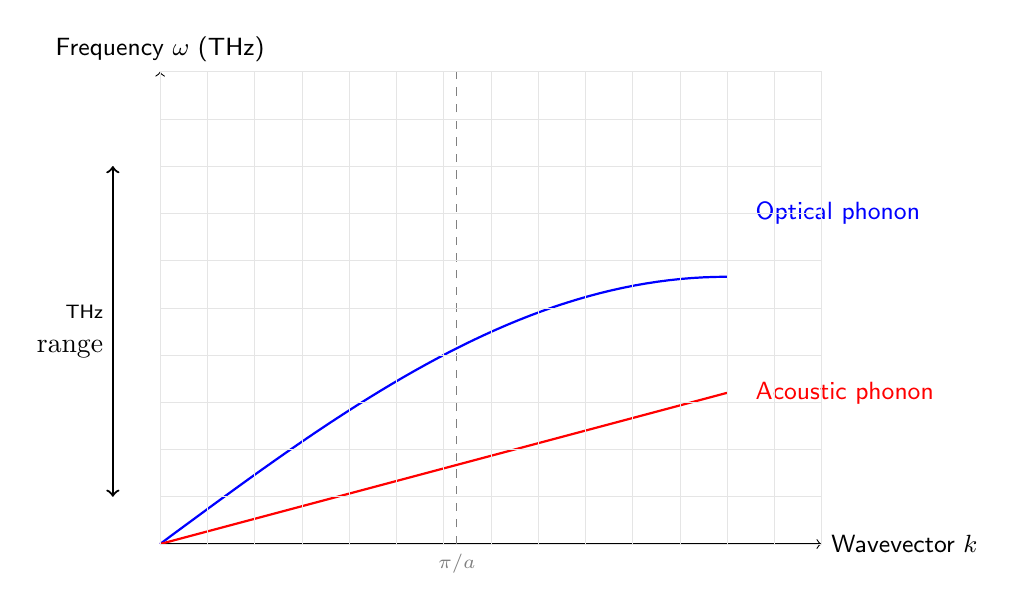
\begin{tikzpicture}[scale=1.2]
% Axes
\draw[->] (0,0) -- (7,0) node[right] {\sffamily\small Wavevector $k$};
\draw[->] (0,0) -- (0,5) node[above] {\sffamily\small Frequency $\omega$ (THz)};

% Draw acoustic phonon branch (linear at low k)
\draw[thick, blue] plot[domain=0:6, samples=50] (\x, {2*sqrt(1-cos(\x*30))});
\node[blue, right] at (6.2, 3.5) {\sffamily\small Optical phonon};

% Draw optical phonon branch (flat)
\draw[thick, red] plot[domain=0:6, samples=50] (\x, {0.8*\x/3});
\node[red, right] at (6.2, 1.6) {\sffamily\small Acoustic phonon};

% Mark first Brillouin zone
\draw[dashed, gray] (3.14, 0) -- (3.14, 5);
\node[below, gray] at (3.14, 0) {\sffamily\scriptsize $\pi/a$};

% THz range annotation
\draw[<->, thick] (-0.5, 0.5) -- (-0.5, 4);
\node[left, align=right] at (-0.5, 2.25) {\sffamily\scriptsize THz\\range};

% Grid
\draw[very thin, gray!20] (0,0) grid[step=0.5] (7,5);
\end{tikzpicture}
\end{center}

\textbf{Implication:} Microtubules support acoustic phonon modes (sound waves along axis) and optical phonon modes (anti-phase oscillations between protofilaments).

\subsection{Acoustic vs. Optical Phonons}
\label{subsec:acoustic-optical}

\textbf{Acoustic phonons:}
\begin{itemize}
\item Adjacent unit cells move in phase
\item Linear dispersion at low $k$: $\omega \propto v_s k$ (sound velocity $v_s \approx 1$--2~km/s in proteins)
\item Low frequency: 0.1--1~THz
\end{itemize}

\textbf{Optical phonons:}
\begin{itemize}
\item Adjacent cells move out of phase
\item Flat dispersion (frequency nearly independent of $k$)
\item Higher frequency: 1--10~THz
\item Couple strongly to EM radiation (IR/THz absorption)
\end{itemize}

\textbf{Microtubule-specific vibrational modes:}
\begin{center}
\begin{tabular}{lll}
\toprule
\textbf{Mode Type} & \textbf{Frequency Range} & \textbf{Description} \\
\midrule
Breathing & $\sim$0.1--0.5~THz & Radial expansion/contraction \\
Bending & $\sim$0.01--0.1~THz & Flexural oscillations (below THz) \\
Longitudinal & $\sim$0.5--2~THz & Compression waves along axis \\
Circumferential & $\sim$1--5~THz & Torsional twisting \\
\bottomrule
\end{tabular}
\end{center}

\begin{center}
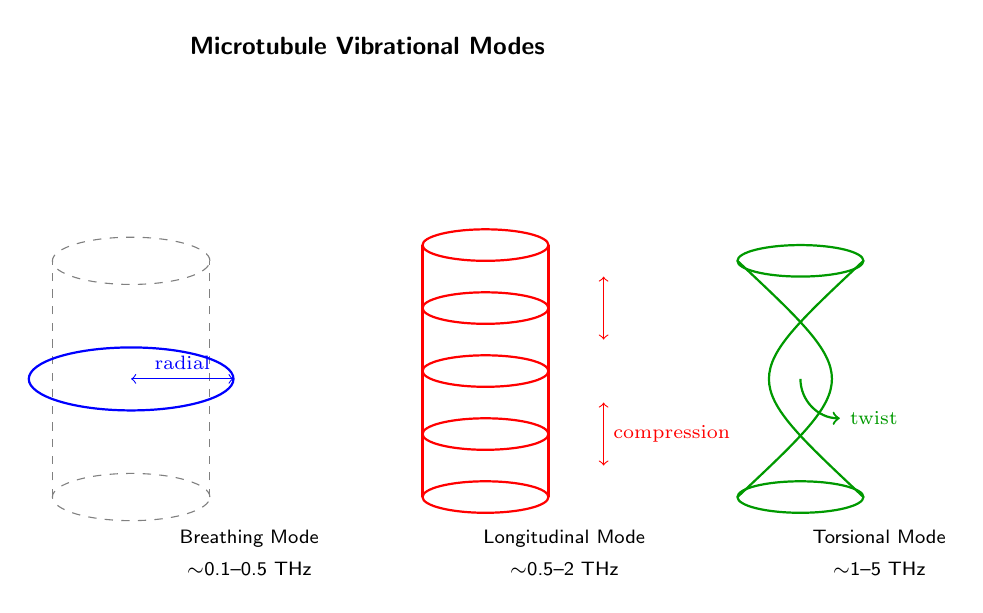
\begin{tikzpicture}[scale=1.0]
% Title
\node[above, font=\sffamily\small\bfseries] at (3, 5.5) {Microtubule Vibrational Modes};

% Breathing mode
\begin{scope}[xshift=0cm]
  \node[below, font=\sffamily\scriptsize] at (1.5, -0.3) {Breathing Mode};
  \node[below, font=\sffamily\scriptsize] at (1.5, -0.7) {$\sim$0.1--0.5 THz};
  % Microtubule at rest (dashed)
  \draw[dashed, gray] (0,0) ellipse (1cm and 0.3cm);
  \draw[dashed, gray] (0,3) ellipse (1cm and 0.3cm);
  \draw[dashed, gray] (-1,0) -- (-1,3);
  \draw[dashed, gray] (1,0) -- (1,3);
  % Expanded state (solid)
  \draw[thick, blue] (0,1.5) ellipse (1.3cm and 0.4cm);
  \draw[<->, blue] (0, 1.5) -- (1.3, 1.5) node[midway, above, font=\scriptsize] {radial};
\end{scope}

% Longitudinal mode
\begin{scope}[xshift=4cm]
  \node[below, font=\sffamily\scriptsize] at (1.5, -0.3) {Longitudinal Mode};
  \node[below, font=\sffamily\scriptsize] at (1.5, -0.7) {$\sim$0.5--2 THz};
  % Microtubule segments
  \foreach \y in {0, 0.8, 1.6, 2.4, 3.2} {
    \draw[thick, red] (0.5,\y) ellipse (0.8cm and 0.2cm);
  }
  \draw[thick, red] (0.5-0.8, 0) -- (0.5-0.8, 3.2);
  \draw[thick, red] (0.5+0.8, 0) -- (0.5+0.8, 3.2);
  % Compression arrows
  \draw[<->, red] (2, 0.4) -- (2, 1.2) node[midway, right, font=\scriptsize] {compression};
  \draw[<->, red] (2, 2.0) -- (2, 2.8);
\end{scope}

% Torsional mode
\begin{scope}[xshift=8cm]
  \node[below, font=\sffamily\scriptsize] at (1.5, -0.3) {Torsional Mode};
  \node[below, font=\sffamily\scriptsize] at (1.5, -0.7) {$\sim$1--5 THz};
  % Microtubule with twist
  \draw[thick, green!60!black] (0.5,0) ellipse (0.8cm and 0.2cm);
  \draw[thick, green!60!black] (0.5,3) ellipse (0.8cm and 0.2cm);
  % Helical lines indicating twist
  \draw[thick, green!60!black] (0.5-0.8, 0) .. controls (0.5+0.8, 1.5) .. (0.5-0.8, 3);
  \draw[thick, green!60!black] (0.5+0.8, 0) .. controls (0.5-0.8, 1.5) .. (0.5+0.8, 3);
  % Rotation arrow
  \draw[->, green!60!black, thick] (0.5, 1.5) arc (180:270:0.5cm) node[right, font=\scriptsize] {twist};
\end{scope}

\end{tikzpicture}
\end{center}


\section{Vibronic Coupling in Tubulin}
\label{sec:vibronic-coupling}

\subsection{What is Vibronic Coupling?}
\label{subsec:vibronic-definition}

\textbf{Vibronic coupling} is the interaction between \textbf{electronic states} and \textbf{vibrational (nuclear) modes}. It is described by the Born-Oppenheimer breakdown term:
\begin{equation}
\label{eq:vibronic-coupling}
H_{\text{coupl}} = \sum_{ij} \langle \Psi_i | \frac{\partial}{\partial Q} | \Psi_j \rangle \cdot \frac{\partial Q}{\partial t}
\end{equation}
where:
\begin{itemize}
\item $\Psi_i$ = electronic wavefunctions
\item $Q$ = nuclear coordinate
\end{itemize}

\textbf{Physical picture:} Vibrations modulate electronic energies $\rightarrow$ electronic transitions drive vibrations (feedback loop).

\subsection{Aromatic Amino Acids as Vibronic Chromophores}\label{aromatic-amino-acids-as-vibronic-chromophores}

Tubulin contains \textbf{aromatic amino acids} (Trp, Tyr, Phe) with $\pi$-electron systems:
\begin{itemize}
\item \textbf{Tryptophan}: 7 per $\alpha$-tubulin, 9 per $\beta$-tubulin
\item \textbf{Tyrosine}: 12 per $\alpha$-tubulin, 13 per $\beta$-tubulin
\item \textbf{Phenylalanine}: 20 per $\alpha$-tubulin, 19 per $\beta$-tubulin
\end{itemize}

These aromatics have:
\begin{itemize}
\item \textbf{Electronic transitions} in UV ($\sim$280 nm, $\sim$1000 THz)
\item \textbf{Vibrational progressions} in THz range (C-C stretches, ring deformations)
\end{itemize}

\textbf{Key point}: UV excitation of aromatics couples to THz lattice vibrations $\rightarrow$ vibronic excitations.

\subsection{Jahn-Teller Effect and Vibronic Stabilization}\label{jahn-teller-effect-and-vibronic-stabilization}

From VE-TFCC quantum chemistry:

\textbf{Jahn-Teller (JT) theorem}: If a molecule has a degenerate
electronic state, it will spontaneously distort to lift the degeneracy.

\textbf{Example from VE-TFCC paper} (CoF$_4^-$):
\begin{itemize}
\item Electronic state $^5E$ (doubly degenerate)
\item JT distortion along $e$ vibrational mode
\item Stabilization energy: \textbf{6 kJ/mol} (comparable to thermal energy at 298 K)
\end{itemize}

\textbf{Biological analogue (speculative)}:
\begin{itemize}
\item Aromatic amino acids in tubulin may have near-degenerate $\pi$-states
\item THz vibrations lift degeneracy $\rightarrow$ vibronic ground state
\item \textbf{Coherence protection}: Vibronic coupling creates avoided crossings that shield quantum superpositions from decoherence
\end{itemize}

\subsection{Thermal Coherence via Bogoliubov Transformation}\label{thermal-coherence-via-bogoliubov-transformation}

From VE-TFCC theory, \textbf{quantum coherence persists at room
temperature} if vibronic coupling is strong enough.

\textbf{Key equations} (from VE-TFCC supporting information):

\textbf{Bogoliubov-transformed operators}:
\begin{equation}
\label{eq:bogoliubov-a}
\hat{a}_i = \frac{1}{\sqrt{1 - e^{-\beta \omega_i}}} \left( \hat{b}_i - e^{-\beta \omega_i/2} \hat{b}_i^\dagger \right)
\end{equation}
\begin{equation}
\label{eq:bogoliubov-a-dag}
\hat{a}_i^\dagger = \frac{1}{\sqrt{1 - e^{-\beta \omega_i}}} \left( \hat{b}_i^\dagger - e^{-\beta \omega_i/2} \hat{b}_i \right)
\end{equation}
where:
\begin{itemize}
\item $\beta = 1/(k_B T)$ = inverse temperature
\item $\omega_i$ = vibrational frequency
\item $\hat{b}_i$ = original Bosonic operators
\end{itemize}

\textbf{Physical meaning}: At temperature \(T\), the thermal state
\(|\theta(\beta)\rangle\) is the \emph{vacuum} for the Bogoliubov
quasiparticles \(\hat{a}_i\).

\textbf{Implication for microtubules}:
\begin{itemize}
\item THz vibrations ($\omega \sim 1$ THz $\approx 48$ K) have $\beta \omega \sim 0.15$ at 310 K
\item Exponential factor $e^{-\beta \omega} \approx 0.86$ (significant thermal population)
\item \textbf{But}: Vibronic coupling can create thermal coherent states if electronic-vibrational coupling is strong
\end{itemize}

\textbf{Position variance} (measure of quantum coherence):
\begin{equation}
\label{eq:position-variance}
(\Delta q_i)^2 = \langle q_i^2 \rangle - \langle q_i \rangle^2
\end{equation}

For a classical thermal system, $(\Delta q)^2 \propto k_B T$. For a vibronic system at thermal equilibrium (from VE-TFCC):
\[(\Delta q_i)^2 = \frac{1}{2} \left( d_{ii}^{bb} + d_{ii}^{aa} + \frac{1}{2} d_{aa}^{bb} + \frac{1}{2} \delta_{aa} \right)\]
where $d^{ab}$ are thermal reduced density matrices in Bogoliubov representation.

\textbf{Key result}: Quantum coherence manifests as \emph{excess
variance} beyond classical thermal prediction.



\section{Experimental Evidence for THz Modes in Microtubules}\label{experimental-evidence-for-thz-modes-in-microtubules}

\subsection{Far-Infrared Spectroscopy}\label{far-infrared-spectroscopy-established}

\textbf{Method}: Fourier-transform infrared (FTIR) spectroscopy in
far-IR/THz range (10-300
cm\textbackslash textsuperscript\{-\}\textbackslash textsuperscript\{1\},
0.3-9 THz)

\textbf{Findings}:
\begin{itemize}
\item \textbf{Absorption peaks} at $\sim$1.5, 3.5, 5.5, 7.2 THz (from dehydrated microtubule samples)
\item Peaks correspond to collective modes (breathing, torsional)
\item Temperature-dependent: Peak positions shift with temperature (anharmonic effects)
\end{itemize}

\textbf{Limitations}:
\begin{itemize}
\item Dehydrated samples (no water); in vivo behavior may differ
\item No phase information (cannot distinguish coherent vs.~incoherent absorption)
\end{itemize}

\textbf{Reference}: Preto (2016), \emph{PLoS ONE} --- First
systematic THz spectroscopy of microtubules

\subsection{Inelastic Neutron Scattering}\label{inelastic-neutron-scattering-established}

\textbf{Method}: Neutrons scatter off vibrating nuclei; energy transfer
measures phonon dispersion \(\omega(k)\)

\textbf{Findings}:
\begin{itemize}
\item Acoustic phonon velocity: $v_s \approx 1.5$ km/s (similar to other proteins)
\item Flat optical phonon branches at 2-8 THz
\item Confirmation of helical symmetry: 13-fold rotational modes
\end{itemize}

\textbf{Limitation}: Requires deuterated samples (exchange H for D); may
alter vibrational spectrum

\textbf{Reference}: Chou et al., \emph{Biophys. J.} (1998) ---
Inelastic scattering on actin (similar protein)

\subsection{Raman Spectroscopy}\label{raman-spectroscopy-established}

\textbf{Method}: Inelastic light scattering; measures vibrational
frequencies via Stokes/anti-Stokes shifts

\textbf{Findings}:
\begin{itemize}
\item Low-frequency Raman (5-100 cm$^{-1}$, 0.15-3 THz) shows collective protein modes
\item \textbf{Boson peak} at $\sim$10 cm$^{-1}$ (0.3 THz): Universal feature of disordered proteins
\item Temperature dependence: Anti-Stokes intensity $\propto n_B(T)$ (Bose-Einstein distribution)
\end{itemize}

\textbf{Limitation}: Cannot probe coherence directly (only measures
energy-level spacing)

\subsection{Terahertz Time-Domain Spectroscopy (THz-TDS)}\label{terahertz-time-domain-spectroscopy-thz-tds-emerging}

\textbf{Method}: Ultrafast THz pulses probe sample; measure transmission
and phase shift

\textbf{Advantages}:
\begin{itemize}
\item Phase-sensitive: Can detect coherent vs.~incoherent response
\item Time-resolved: Sub-picosecond resolution (can track coherence decay)
\end{itemize}

\textbf{Current status}:
\begin{itemize}
\item THz-TDS on proteins is emerging
\item Few studies on microtubules specifically
\item Technical challenge: Water absorption in THz range (biological samples)
\end{itemize}

\textbf{Needed experiment}: THz-TDS on hydrated microtubules at 310 K to measure:
\begin{itemize}
\item Coherence time $\tau_c$
\item Phonon lifetime $\tau_p$
\item Vibronic coupling strength
\end{itemize}



\section{Theoretical Models}\label{theoretical-models}

\subsection{Fröhlich Condensate Model (1968)}\label{fruxf6hlich-condensate-model-1968}

\textbf{Herbert Fröhlich} proposed that biological systems can exhibit
\textbf{phonon condensation}---a Bose-Einstein-like condensate of
coherent vibrations.

\textbf{Mechanism}:
\begin{enumerate}
\item Metabolic energy pumps THz phonons (non-equilibrium)
\item If pumping rate $>$ damping rate, phonons accumulate in lowest mode
\item Coherent macroscopic oscillation emerges
\end{enumerate}

\textbf{Fröhlich frequency} (predicted): $\omega_F \sim 10^{11}$ Hz = 0.1 THz

\textbf{Criticisms}:
\begin{itemize}
\item Requires extreme non-equilibrium (metabolic rates insufficient?)
\item Decoherence from water and ions
\end{itemize}

\textbf{Modern revival}: Some experiments claim to detect Fröhlich
condensation in proteins (controversial)

\subsection{Davydov Soliton Model (1973)}\label{davydov-soliton-model-1973}

\textbf{Amide-I band} (C=O stretch in protein backbone, $\sim$1650 cm$^{-1}$, 50 THz) can form \textbf{solitons}---self-trapped localized excitations.

\textbf{Mechanism}:
\begin{itemize}
\item Exciton (electronic excitation) couples to lattice (phonon)
\item Exciton creates local lattice distortion
\item Distortion traps exciton $\rightarrow$ stable traveling wave (soliton)
\end{itemize}

\textbf{Relevance to microtubules}:
\begin{itemize}
\item If aromatic $\pi$-excitations couple to THz phonons, similar solitons could exist
\item \textbf{Energy transport}: Solitons could carry energy along microtubule without dissipation
\end{itemize}

\textbf{Problem}: Room-temperature stability questionable (thermal
fluctuations disrupt solitons)

\subsection{Vibronic Exciton Model (Modern)}\label{vibronic-exciton-model-modern}

\textbf{Combines}: Fröhlich (phonons) + Davydov (excitons) + VE-TFCC
(thermal coherence)

\textbf{Hamiltonian}:
\begin{equation}
\label{eq:vibronic-hamiltonian}
\hat{H} = \underbrace{\sum_i \epsilon_i | i \rangle \langle i |}_{\text{Electronic}} + \underbrace{\sum_k \hbar \omega_k \hat{b}_k^\dagger \hat{b}_k}_{\text{Vibrational}} + \underbrace{\sum_{ik} g_{ik} | i \rangle \langle i | (\hat{b}_k + \hat{b}_k^\dagger)}_{\text{Vibronic coupling}}
\end{equation}
where:
\begin{itemize}
\item $| i \rangle$ = electronic states (localized on tubulin dimers)
\item $\hat{b}_k$ = phonon operators
\item $g_{ik}$ = vibronic coupling strength
\end{itemize}

\textbf{At thermal equilibrium} (VE-TFCC approach):
\begin{itemize}
\item Transform to Bogoliubov representation: $\hat{b}_k \rightarrow \hat{a}_k$
\item Thermal state $|\theta(\beta)\rangle$ becomes vacuum for $\hat{a}_k$
\item Coherent thermal excitations survive if $g_{ik}$ is large enough
\end{itemize}

\textbf{Prediction}: If $g_{ik} \omega_k \gtrsim k_B T$, vibronic states maintain quantum coherence at 310 K.

\textbf{Estimate for microtubules}:
\begin{itemize}
\item $\omega_k \sim 1$ THz $\rightarrow \hbar \omega_k \approx 4$ meV
\item $k_B T$ (310 K) $\approx 27$ meV
\item Need $g_{ik} \gtrsim 7$ for thermal coherence
\end{itemize}

\textbf{Question}: Is vibronic coupling in tubulin this strong?
Unknown---requires detailed quantum chemistry calculations (VE-TFCC
on tubulin model).


\subsection{Worked Example: Phonon Propagation Speed}
\label{subsec:worked-example}

\begin{calloutbox}{Worked Example: Signal Transit Time Along Microtubule}
\textbf{Problem:} Calculate the time for an acoustic phonon to travel along a 10~$\mu$m microtubule segment.

\textbf{Given:}
\begin{itemize}
\item Microtubule length: $L = 10~\mu$m $= 10 \times 10^{-6}$~m
\item Sound velocity in protein: $v_s \approx 1.5$~km/s $= 1500$~m/s
\end{itemize}

\textbf{Solution:}

Transit time is:
\begin{equation}
t = \frac{L}{v_s} = \frac{10 \times 10^{-6}~\text{m}}{1500~\text{m/s}} = 6.67 \times 10^{-9}~\text{s} = \mathbf{6.7~\text{ns}}
\end{equation}

\textbf{Comparison with diffusion:}

For a small molecule diffusing along the same distance with diffusion coefficient $D \approx 10^{-10}$~m$^2$/s:
\begin{equation}
t_{\text{diff}} \approx \frac{L^2}{2D} = \frac{(10^{-5})^2}{2 \times 10^{-10}} = 0.5~\text{s}
\end{equation}

\textbf{Conclusion:} Phonon propagation is \textbf{$\sim$75 million times faster} than molecular diffusion over microtubule lengths, suggesting a potential mechanism for rapid long-range signaling.
\end{calloutbox}



\section{Potential Biological Functions}\label{potential-biological-functions-speculative}

\subsection{Quantum Information Processing}\label{quantum-information-processing}

\textbf{Hypothesis}: Microtubules act as quantum waveguides for
information processing in neurons.

\textbf{Mechanism}:
\begin{itemize}
\item Tubulin dimers in superposition: $|\psi\rangle = \alpha|\uparrow\rangle + \beta|\downarrow\rangle$
\item THz phonons mediate entanglement between distant tubulins
\item Quantum coherence spans $\sim$10 $\mu$m (length of microtubule segment)
\end{itemize}

\textbf{Requirements}:
\begin{itemize}
\item Coherence time $\tau_c > 1$ ms (gamma oscillation timescale)
\item Isolation from thermal bath (ordered water?)
\item Amplification mechanism (connect to action potentials?)
\end{itemize}

\textbf{Current status}: No experimental evidence; coherence time estimates range from 10 fs (skeptics) to 10 ms (proponents).

\subsection{Long-Range Signaling}\label{long-range-signaling}

\textbf{Non-quantum version}: Coherent phonons propagate along microtubule, modulating tubulin-associated protein (TAP) binding.

\textbf{Phonon propagation speed}: $v_s \approx 1.5$ km/s

\textbf{Microtubule length}: $\sim$10 $\mu$m (typical)

\textbf{Transit time}: $\sim$7 ns (much faster than diffusion)

\textbf{Possible function}: Coordinate motor protein activity (kinesin,
dynein) along entire microtubule.

\textbf{Evidence}: Indirect---motor proteins have been shown to
respond to mechanical vibrations in vitro.

\subsection{Anesthetic Sensitivity}\label{anesthetic-sensitivity}

\textbf{Clinical observation}: General anesthetics (isoflurane,
propofol) bind to microtubules and disrupt consciousness.

\textbf{Quantum hypothesis}: Anesthetics disrupt THz vibronic coherence $\rightarrow$ loss of quantum information processing $\rightarrow$ unconsciousness.

\textbf{Alternative (classical)}: Anesthetics alter microtubule mechanics $\rightarrow$ disrupt synaptic transmission (no quantum effects needed).

\textbf{Test}: Does THz spectroscopy of microtubules change upon
anesthetic binding? - \textbf{Preliminary data} (in vitro): Anesthetics
shift THz absorption peaks by $\sim$0.1 THz - \textbf{In vivo
test}: Not yet performed




\section{Applications and Experimental Techniques}
\label{sec:applications}

\subsection{Far-Infrared Spectroscopy of Microtubules}
\label{subsec:app-ftir}

\textbf{Technique:} Fourier-transform infrared (FTIR) spectroscopy in the far-IR/THz range (10--300~cm$^{-1}$, 0.3--9~THz).

\textbf{Key Results:}
\begin{itemize}
\item Absorption peaks at $\sim$1.5, 3.5, 5.5, 7.2~THz in dehydrated microtubule samples
\item Peaks correspond to collective vibrational modes (breathing, torsional)
\item Temperature-dependent peak shifts reveal anharmonic effects
\end{itemize}

\begin{warningbox}
\textbf{Critical Limitation:} Most THz spectroscopy studies use dehydrated samples due to strong water absorption in the THz range. In vivo behavior may differ significantly from measurements in vacuum or dry conditions.
\end{warningbox}

\textbf{Reference:} Preto (2016), \textit{PLoS ONE}---First systematic THz spectroscopy of microtubules.

\subsection{Terahertz Time-Domain Spectroscopy (THz-TDS)}
\label{subsec:app-thz-tds}

\textbf{Advantages over conventional FTIR:}
\begin{itemize}
\item \textbf{Phase-sensitive:} Can detect coherent vs. incoherent response
\item \textbf{Time-resolved:} Sub-picosecond resolution tracks coherence decay
\item \textbf{Direct field measurement:} Measures electric field amplitude and phase
\end{itemize}

\textbf{Current Status:} Emerging technology for biological samples; few studies on microtubules specifically.

\textbf{Future Potential:} THz-TDS on hydrated microtubules at 310~K could measure:
\begin{itemize}
\item Coherence time $\tau_c$
\item Phonon lifetime $\tau_p$  
\item Vibronic coupling strength
\end{itemize}

\subsection{Anesthetic Interaction Studies}
\label{subsec:app-anesthetics}

\textbf{Clinical Observation:} General anesthetics (isoflurane, propofol) bind to microtubules and disrupt consciousness.

\begin{calloutbox}{Experimental Protocol}
\textbf{Test for functional role of THz coherence:}

\begin{enumerate}
\item Measure THz spectrum of microtubules \textit{in vitro} (baseline)
\item Add anesthetic (isoflurane) $\rightarrow$ remeasure spectrum
\item Quantify:
  \begin{itemize}
  \item Shifts in resonance frequencies ($\Delta\omega$)
  \item Changes in coherence time ($\Delta\tau_c$)
  \item Changes in absorption intensity
  \end{itemize}
\item Remove anesthetic $\rightarrow$ verify reversibility
\end{enumerate}

\textbf{Prediction (if THz coherence is functionally relevant):} Anesthetic should reduce $\tau_c$ or shift resonance frequencies by $\sim$0.1~THz.

\textbf{Preliminary Data:} Anesthetics shift THz absorption peaks by $\sim$0.1~THz \textit{in vitro}. \textit{In vivo} tests not yet performed.
\end{calloutbox}

\section{Challenges to THz Quantum Coherence}\label{challenges-to-thz-quantum-coherence}

\subsection{Decoherence from Water}\label{decoherence-from-water}

\textbf{Problem}: Water has strong THz absorption (rotational modes at
0.1-3 THz).

\textbf{Decoherence time estimate}:
\begin{equation}
\label{eq:decoherence-time}
\tau_d \sim \frac{\hbar}{\Gamma k_B T}
\end{equation}
where $\Gamma$ is the system-bath coupling. For microtubules in water, $\Gamma \sim 10^{12}$~s$^{-1}$ $\rightarrow \tau_d \sim 100$~fs.

\textbf{Counter-argument}: Ordered water layers near microtubule surface may have reduced rotational freedom $\rightarrow$ weaker coupling.

\textbf{Evidence}: Neutron scattering shows water within 1 nm of protein
surfaces has restricted dynamics (residence time $\sim$10 ps
vs.~$\sim$1 ps in bulk).

\subsection{Thermal Energy Dominates}\label{thermal-energy-dominates}

\textbf{At 310 K}: $k_B T \approx 27$ meV $\gg \hbar \omega$ (1 THz) $\approx 4$ meV.

\textbf{Classical expectation}: Thermal occupation number $n_B(T) = (\exp(\hbar \omega / k_B T) - 1)^{-1} \approx 5.7$ (many phonons thermally excited).

\textbf{Quantum coherence destroyed?} Not necessarily---VE-TFCC shows that vibronic coupling can maintain \emph{thermal coherent states} even with $n_B \gg 1$.

\textbf{Key distinction}: - \textbf{Classical thermal state}: Incoherent
mixture of phonon number states - \textbf{Thermal coherent state}:
Superposition with well-defined phase (enabled by vibronic coupling)

\subsection{Lack of Experimental Proof}\label{lack-of-experimental-proof}

\textbf{Critical issue}: No experiment has directly demonstrated:
\begin{itemize}
\item Sub-millisecond quantum coherence in microtubules at 310 K
\item Functional role of THz coherence in living neurons
\item Quantum advantage for any biological computation
\end{itemize}

\textbf{What's needed}:
\begin{itemize}
\item THz-TDS on functioning neurons (technical challenge)
\item Two-dimensional THz spectroscopy (detect off-diagonal coherences)
\item Conditional coherence measurements (if coherence exists, disrupting it should alter function)
\end{itemize}



\section{Future Experiments}\label{future-experiments}

\subsection{Two-Dimensional THz Spectroscopy}\label{two-dimensional-thz-spectroscopy}

\textbf{Method}: Send two THz pulses separated by delay $\tau$; measure response as function of $\tau$.

\textbf{What it measures}: Off-diagonal elements of density matrix $\rho_{ij}$ (coherences between states $i$ and $j$).

\textbf{Signature of quantum coherence}: Oscillatory beats in 2D spectrum with decay time $\tau_c$.

\textbf{Challenge}: Requires intense, phase-stable THz sources
(free-electron lasers or table-top THz systems).

\subsection{Quantum Coherence Tomography}\label{quantum-coherence-tomography}

\textbf{Idea}: Use microtubule-specific fluorescent probes that report
on vibronic coupling strength.

\textbf{Mechanism}: Probe's fluorescence lifetime depends on local phonon density of states $\rightarrow$ map coherence spatially.

\textbf{Proof-of-concept}: Similar techniques used in photosynthetic
complexes.

\subsection{Anesthetic Modulation Studies}\label{anesthetic-modulation-studies}

\textbf{Protocol}:
\begin{enumerate}
\item Measure THz spectrum of microtubules in vitro (no anesthetic)
\item Add anesthetic (isoflurane) $\rightarrow$ remeasure
\item Compare coherence times and spectral shifts
\end{enumerate}

\textbf{Prediction} (if THz coherence is functionally relevant):
\begin{itemize}
\item Anesthetic should reduce $\tau_c$ or shift resonance frequencies
\item Reversible upon anesthetic removal
\end{itemize}




\section{Summary}
\label{sec:summary}

THz resonances in microtubules represent an established physical phenomenon with speculative biological implications:

\subsection{What We Know (Established)}

\begin{itemize}
\item \textbf{Phonon modes exist:} Far-IR spectroscopy, Raman, and neutron scattering confirm collective vibrational modes at 0.1--10~THz
\item \textbf{Dispersion relations:} Acoustic and optical phonon branches follow predicted dispersion (Equation~\ref{eq:phonon-dispersion})
\item \textbf{Multiple mode types:} Breathing ($\sim$0.1--0.5~THz), longitudinal ($\sim$0.5--2~THz), and torsional ($\sim$1--5~THz) modes identified
\item \textbf{Fast propagation:} Phonons travel at $\sim$1.5~km/s, enabling nanosecond-scale signaling over microtubule lengths
\end{itemize}

\subsection{What Remains Speculative}

\begin{itemize}
\item \textbf{Quantum coherence at 310~K:} Whether vibronic coupling (Section~\ref{sec:vibronic-coupling}) can maintain thermal coherent states is unproven
\item \textbf{Biological function:} No direct evidence that THz resonances play functional roles in neurons or consciousness
\item \textbf{Decoherence times:} Conflicting estimates range from 100~fs to 10~ms; \textit{in vivo} measurements needed
\item \textbf{Anesthetic mechanism:} Correlation between microtubule binding and consciousness disruption is suggestive but not mechanistically understood
\end{itemize}

\subsection{Key Challenges}

\begin{enumerate}
\item \textbf{Water absorption:} THz waves are strongly absorbed by water, making \textit{in vivo} measurements difficult
\item \textbf{Thermal fluctuations:} At $k_B T \approx 27$~meV (310~K), thermal energy exceeds typical THz photon energies ($\sim$4~meV at 1~THz)
\item \textbf{Experimental limitations:} Most studies use dehydrated samples; biological relevance unclear
\end{enumerate}

\subsection{Future Directions}

Critical experiments needed:
\begin{itemize}
\item THz time-domain spectroscopy on hydrated microtubules at 310~K
\item Two-dimensional THz spectroscopy to detect off-diagonal coherences
\item Conditional measurements: disrupt putative THz coherence and observe functional changes
\item Anesthetic modulation studies correlating spectral shifts with consciousness disruption
\end{itemize}

\begin{keyconcept}
\textbf{Bottom Line:} THz resonances in microtubules are real, measurable, and theoretically interesting. Whether they serve functional biological roles---especially in consciousness---remains an open question requiring direct experimental tests.
\end{keyconcept}

\section{Connections to Other Topics}\label{connections-to-other-wiki-pages}

\begin{itemize}

\item
  \textbf{Quantum Coherence in Biological Systems:} --- General
  framework for biological quantum effects
\item
  \textbf{Microtubule Structure and Function:} --- Structural
  basis for THz modes
\item
  \textbf{Orchestrated Objective Reduction (Orch-OR):} ---
  Consciousness theory requiring microtubule coherence
\item
  \textbf{Terahertz (THz) Technology:} --- Experimental tools for
  probing THz resonances
\item
  \textbf{THz Propagation in Biological Tissue:} --- How THz waves
  interact with tissue
\end{itemize}



\section{References}\label{references}

\subsection{Theoretical Foundations}\label{theoretical-foundations}

\begin{enumerate}
\def\labelenumi{\arabic{enumi}.}

\item
  \textbf{Bao et al., \emph{J. Chem. Theory Comput.} 20, 4377 (2024)}
  --- VE-TFCC theory: thermal vibronic coherence
\item
  \textbf{Fröhlich, \emph{Int. J. Quantum Chem.} 2, 641 (1968)} ---
  Original Fröhlich condensate proposal
\item
  \textbf{Davydov, \emph{J. Theor. Biol.} 38, 559 (1973)} ---
  Soliton model in proteins
\end{enumerate}

\subsection{Experimental Studies}\label{experimental-studies}

\begin{enumerate}
\def\labelenumi{\arabic{enumi}.}
\setcounter{enumi}{3}

\item
  \textbf{Preto, \emph{PLoS ONE} 11, e0157267 (2016)} --- THz
  spectroscopy of microtubules
\item
  \textbf{Chou et al., \emph{Biophys. J.} 74, 3317 (1998)} ---
  Inelastic neutron scattering on proteins
\item
  \textbf{Reimers et al., \emph{Proc. Natl. Acad. Sci.} 106, 4219
  (2009)} --- Water structure near proteins
\end{enumerate}

\subsection{Critical Assessments}\label{critical-assessments}

\begin{enumerate}
\def\labelenumi{\arabic{enumi}.}
\setcounter{enumi}{6}

\item
  \textbf{Tegmark, \emph{Phys. Rev.~E} 61, 4194 (2000)} ---
  Skeptical: decoherence too fast in microtubules
\item
  \textbf{Koch \& Hepp, \emph{Nature} 440, 611 (2006)} --- Critique
  of quantum brain theories
\end{enumerate}

\subsection{Anesthesia Connection}\label{anesthesia-connection}

\begin{enumerate}
\def\labelenumi{\arabic{enumi}.}
\setcounter{enumi}{8}

\item
  \textbf{Turin \& Skoulakis, \emph{Proc. Natl. Acad. Sci.} 115, E3524
  (2018)} --- Anesthetics and quantum effects
\end{enumerate}



\textbf{Last updated}: October 2025
